\documentclass{article}
\usepackage[spanish]{babel}
\usepackage[utf8]{inputenc}
\usepackage[nonatbib]{../template}

\usepackage[utf8]{inputenc} % allow utf-8 input
\usepackage[T1]{fontenc}    % use 8-bit T1 fonts
\usepackage{hyperref}       % hyperlinks
\usepackage{url}            % simple URL typesetting
\usepackage{booktabs}       % professional-quality tables
\usepackage{amsfonts}       % blackboard math symbols
\usepackage{nicefrac}       % compact symbols for 1/2, etc.
\usepackage{microtype}      % microtypography
\usepackage{xcolor}         % colors
\usepackage{graphicx}
\usepackage{float}
\usepackage[backend=biber,sorting=ynt,style=apa]{biblatex}

\addbibresource{../bibliography.bib}

\graphicspath{ {../imagenes/} }

\title{Entrega 2: Metodología y EDA}

\author{%
  José Saint Germain\\
  \texttt{josesg998@gmail.com} \\
}

\begin{document}

\maketitle

\section{Introducción}
El objetivo de esta entrega es realizar una breve descripción de las metodologías 
que se utilizarán durante el trabajo final de especialización, así como realizar 
un análisis exploratorio de los datos (EDA), para comprender mejor la estructura 
de los datos que se trabajarán.

\section{Metodología}
Como lo que buscamos realizar es experimentar con diferentes datos el mismo 
trabajo realizado por el FMI (\cite{Ceb24}), vamos a replicar las mismas 
técnicas de optimización de hiperparámetros, así como los mismos algoritmos
de entrenamiento y de intepretación de resultados.
 
% TODO incluyo explicación de los algoritmos?
Los algoritmos que se utilizarán serán Random Forest (\cite{Bre01}) y XGBoost
(\cite{Che16}). Adicionalmente, para la evaluación de performance se utilizará 
el área bajo la curva (AUC), en donde un valor de AUC de 0.5 indica que el modelo 
no tiene capacidad predictiva, mientras que un valor cercano a 1 indica que el 
modelo es capaz de predecir con alta precisión. 

Con respecto al ajuste de hiperparámetros se utilizará la optimización bayesiana.
La misma consistirá en 100 iteraciones en donde se buscará el valor óptimo de los
siguientes hiperparámetros:

% agregar lista de viñetas
\begin{itemize}
  \item Random Forest: profundidad máxima de los árboles (max\_depth) y la 
  submuestra del ratio de columnas a considerar cuando se construye cada árbol 
  (max\_features).
  \item XGBoost: la tasa de aprendizaje (learning\_rate) y el término de 
  regularización L2 en los pesos (reg\_lambda).
\end{itemize}

Adicionalmente el parámetro que establece la cantidad de árboles creados 
(n\_estimators) quedará fijado en 1000.

Para evitar el data leakage, en cada iteraciónd de la optimización bayesiana
se utilizará la validacón cruzada. Sin embargo, como se trabajará con una base
de datos de panel, conviene utilizar una versión adaptada: el método \textit{block-
time-series cross-validation}, basado en \cite{Bur94} y \cite{RAc00}. El método 
aplicado en este caso consiste en generar 5 pares de entrenamiento y validación: 
{1970 - 2009, 2010 - 2011}; {1970 - 2011, 2012 - 2013}; {1970 - 2013, 2014 - 2015}; 
{1970 - 2015, 2016 - 2017}; {1970 - 2017, 2018- 2019}. Por lo tanto, cada set de 
entrenamiento consiste en observaciones desde 1970 hasta un añ de corte (2009, 
2011, 2013, 2015, 2017) y el set de validación contempla los dos años siguientes 
del mismo.

% TODO incluir explicacíón de los Shapley Values
Una vez realizada la optimización bayesiana, se toman los valores de hiperparámetros
que lograron maximizar el AUC y se entrena el modelo con el set de entrenamiento para
intentar predecir los golpes de estado entre 2020 y 2022. Por último, para intepretar
las variables más importantes en la predicción de golpes de estado, se utilizarán los
valores Shapley (\cite{Str10}; \cite{Lun17}). Basado en la teoría de juegos, los
valores Shapley buscan medir la contribución de cada predictor aa la probabilidad de
un golpe en relación con la probabilidad promedio de la muestra prevista de un golpe.

\section{Análisis Exploratorio de Datos}

Como descripción general de la base de datos de VDEM (\cite{Cop24}), podemos 
mencionar que cuenta con 27734 filas y 4607 columnas. Como es una base de datos 
de panel, se tiene información de 202 países durante 235 años. Para comprender la 
estructura de la información, es importante destacar que la base original cuenta 
con información brindada por distintos expertos para cada país en cada año. Para 
poder procesar y obtener la base final, se agrega la información de diferentes 
maneras. Es por este motivo que, además de la información identificactoria de 
cada país (la cual se repite en cada año), la mayoría de las variables sustantivas 
cuentan con diferentes versiones, por cada tipo de variable de agregación generada. 
Por ejemplo, una variable puede contar con su versión princial, la cual es un 
promedio reescalado del 1 al 5, sumado a una versión con la media simple (con 
sufijo \_mean); una versión con el valor máximo y mínimo expresado por un experto 
(\_codehigh y \ codelow, respectivamente); y una versión con el desvío estándar 
(\_sd), en caso de buscar conocer el grado de 'acuerdo' entre los expertos respecto 
a la situación del país.

A la base original obtenida desde la librería de VDEM, se le realizaron los
siguientes filtros: en primer lugar, se removieron todas las variables que
no sean las principales, es decir, que no cuenten con sufijo. De esa manera,
se busca reducir el tamaño de la base y así poder agregar nuevas columnas
mediante ingeniería de atributos. En segundo lugar, se filtraron los años 
superiores a 1950, para adecuarnos al periodo utilizado en el artiçulo del FMI.
De esa manera, la base filtrada cuenta con 12208 filas y 1460 columnas.
%TODO chequear si  voy a seguir filtrando cosas

\subsection{Ánalisis de nulos}
Debido a la alta cantidad de variables, no es posible realizar un análisis
pormenorizado de la presencia de nulos en cada una. Por ese motivo, se decidió
visualizar la misma mediante los agrupadores de variables con las que cuenta el
codebook de VDEM. El mismo, discrimina las variables a partir de sus temas en común.
De esa manera, en la figura 1 la cantidad de nulos por categoría de variable
expresado en un mapa de calor, donde cada fila es una variable individual y las
columnas los diferentes años del panel.

\begin{figure}[H]
  \centering  
  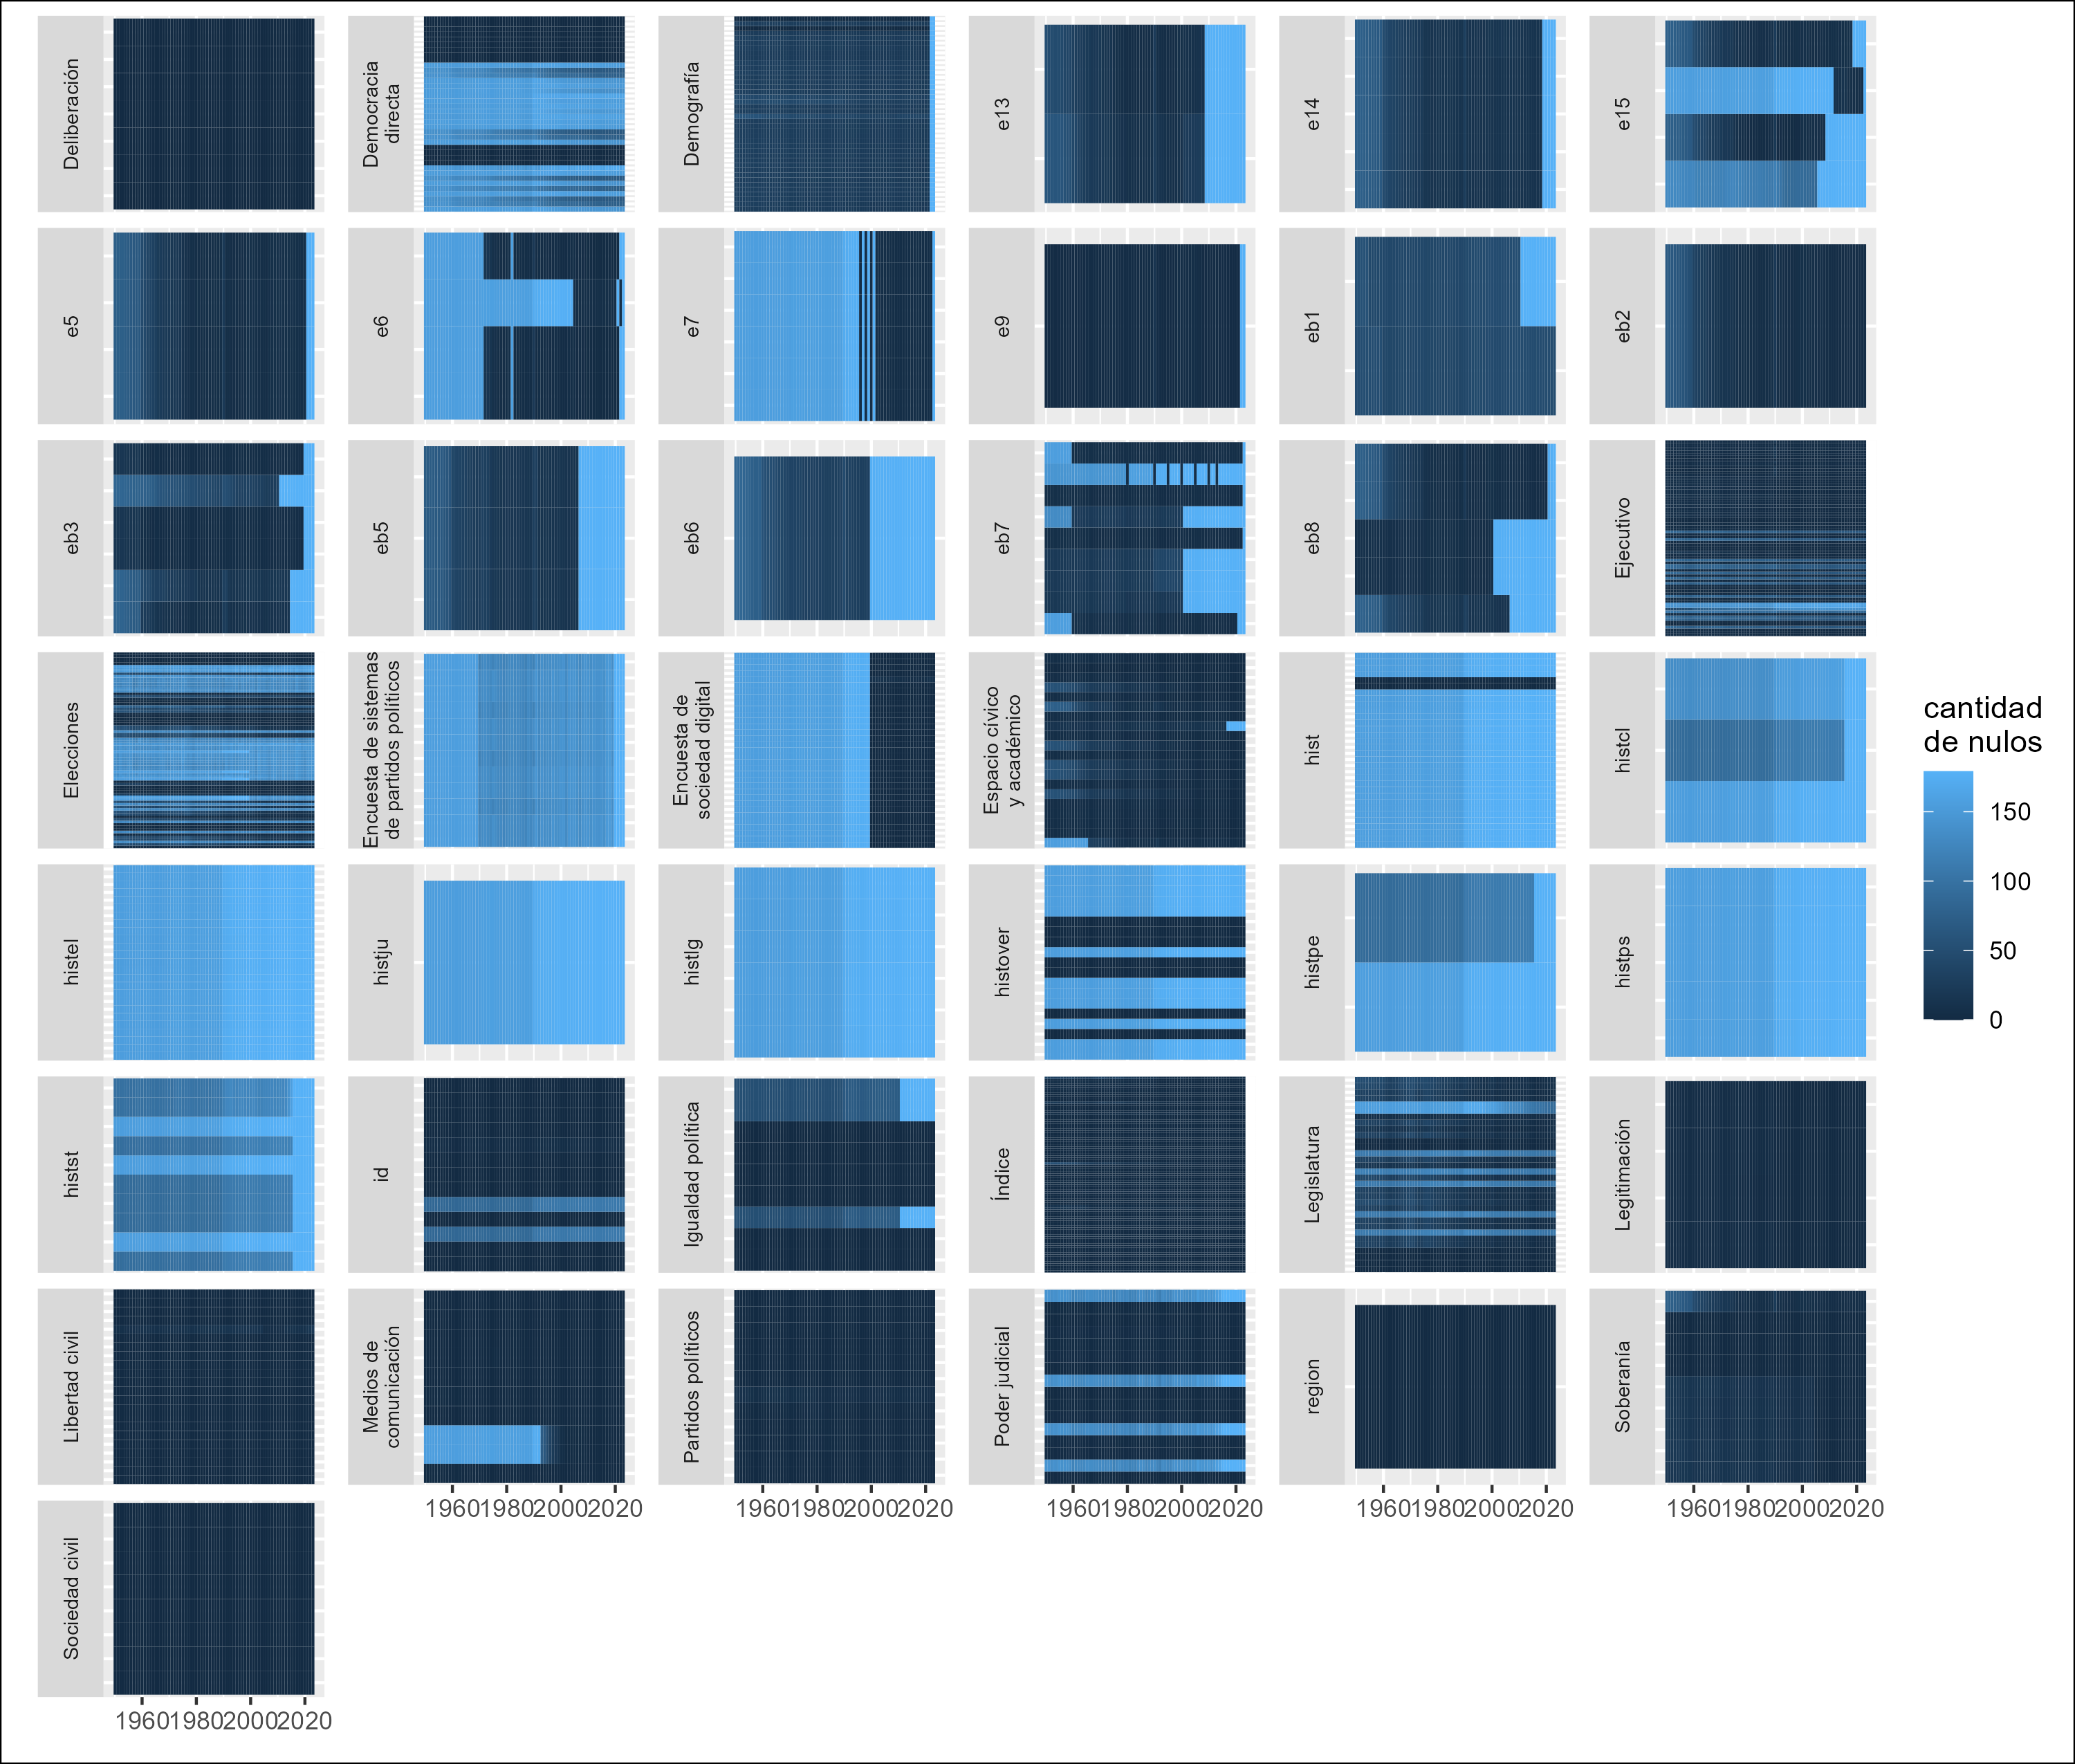
\includegraphics[width=1\textwidth]{1_nas.png}
  \caption{Conteo de nulos por año y agrupador de variables}
\end{figure}

De este gráfico podemos aprehender ciertos patrones sobre la presencia de nulos
en algunos grupos de variables: En primer lugar, observamos variables que,
anteriormente a un año puntual, no cuentan con información. En este ejemplo caen
las variables sobre governanza otorgadas por el banco mundial (e7), las preguntas
pertenecientes a la encuesta de sociedad digital (wsmcio), variables referentes a
la libertad en medios digitales (wsmdmf), las referntes a la polarización en medios
online (wsmomp) y las referentes a clivajes sociales (wsmsc).

En segundo lugar, figuran casos contrarios, en donde a partir de determinado año
la cantidad de datos faltantes salta a la totalidad de los casos. En este grupo
figuran las variables asociadas a instituciones y eventos políticos (e13), cuya 
fuente es un artículo de Przeworski de 2013; las variables cuya fuente es la base
de datos polity V (e14); las variables sobre educación (aumentan los nulos en algunas 
variables) (eb1); las variables sobre recursos naturales (eb5), cuya fuente tiene
datos hasta 2006; las variables sobre infraestructura (eb6); y las relacionadas a 
conflictos (eb8). En general, esta discontinuidad sucede debido a que la información
de estas variables provienen de fuentes externas no gestionadas por VDEM, las cuales
finalizaron su serie en un año puntual.

\subsection{Análisis de variable objetivo}

\begin{figure}[H]
  \centering  
  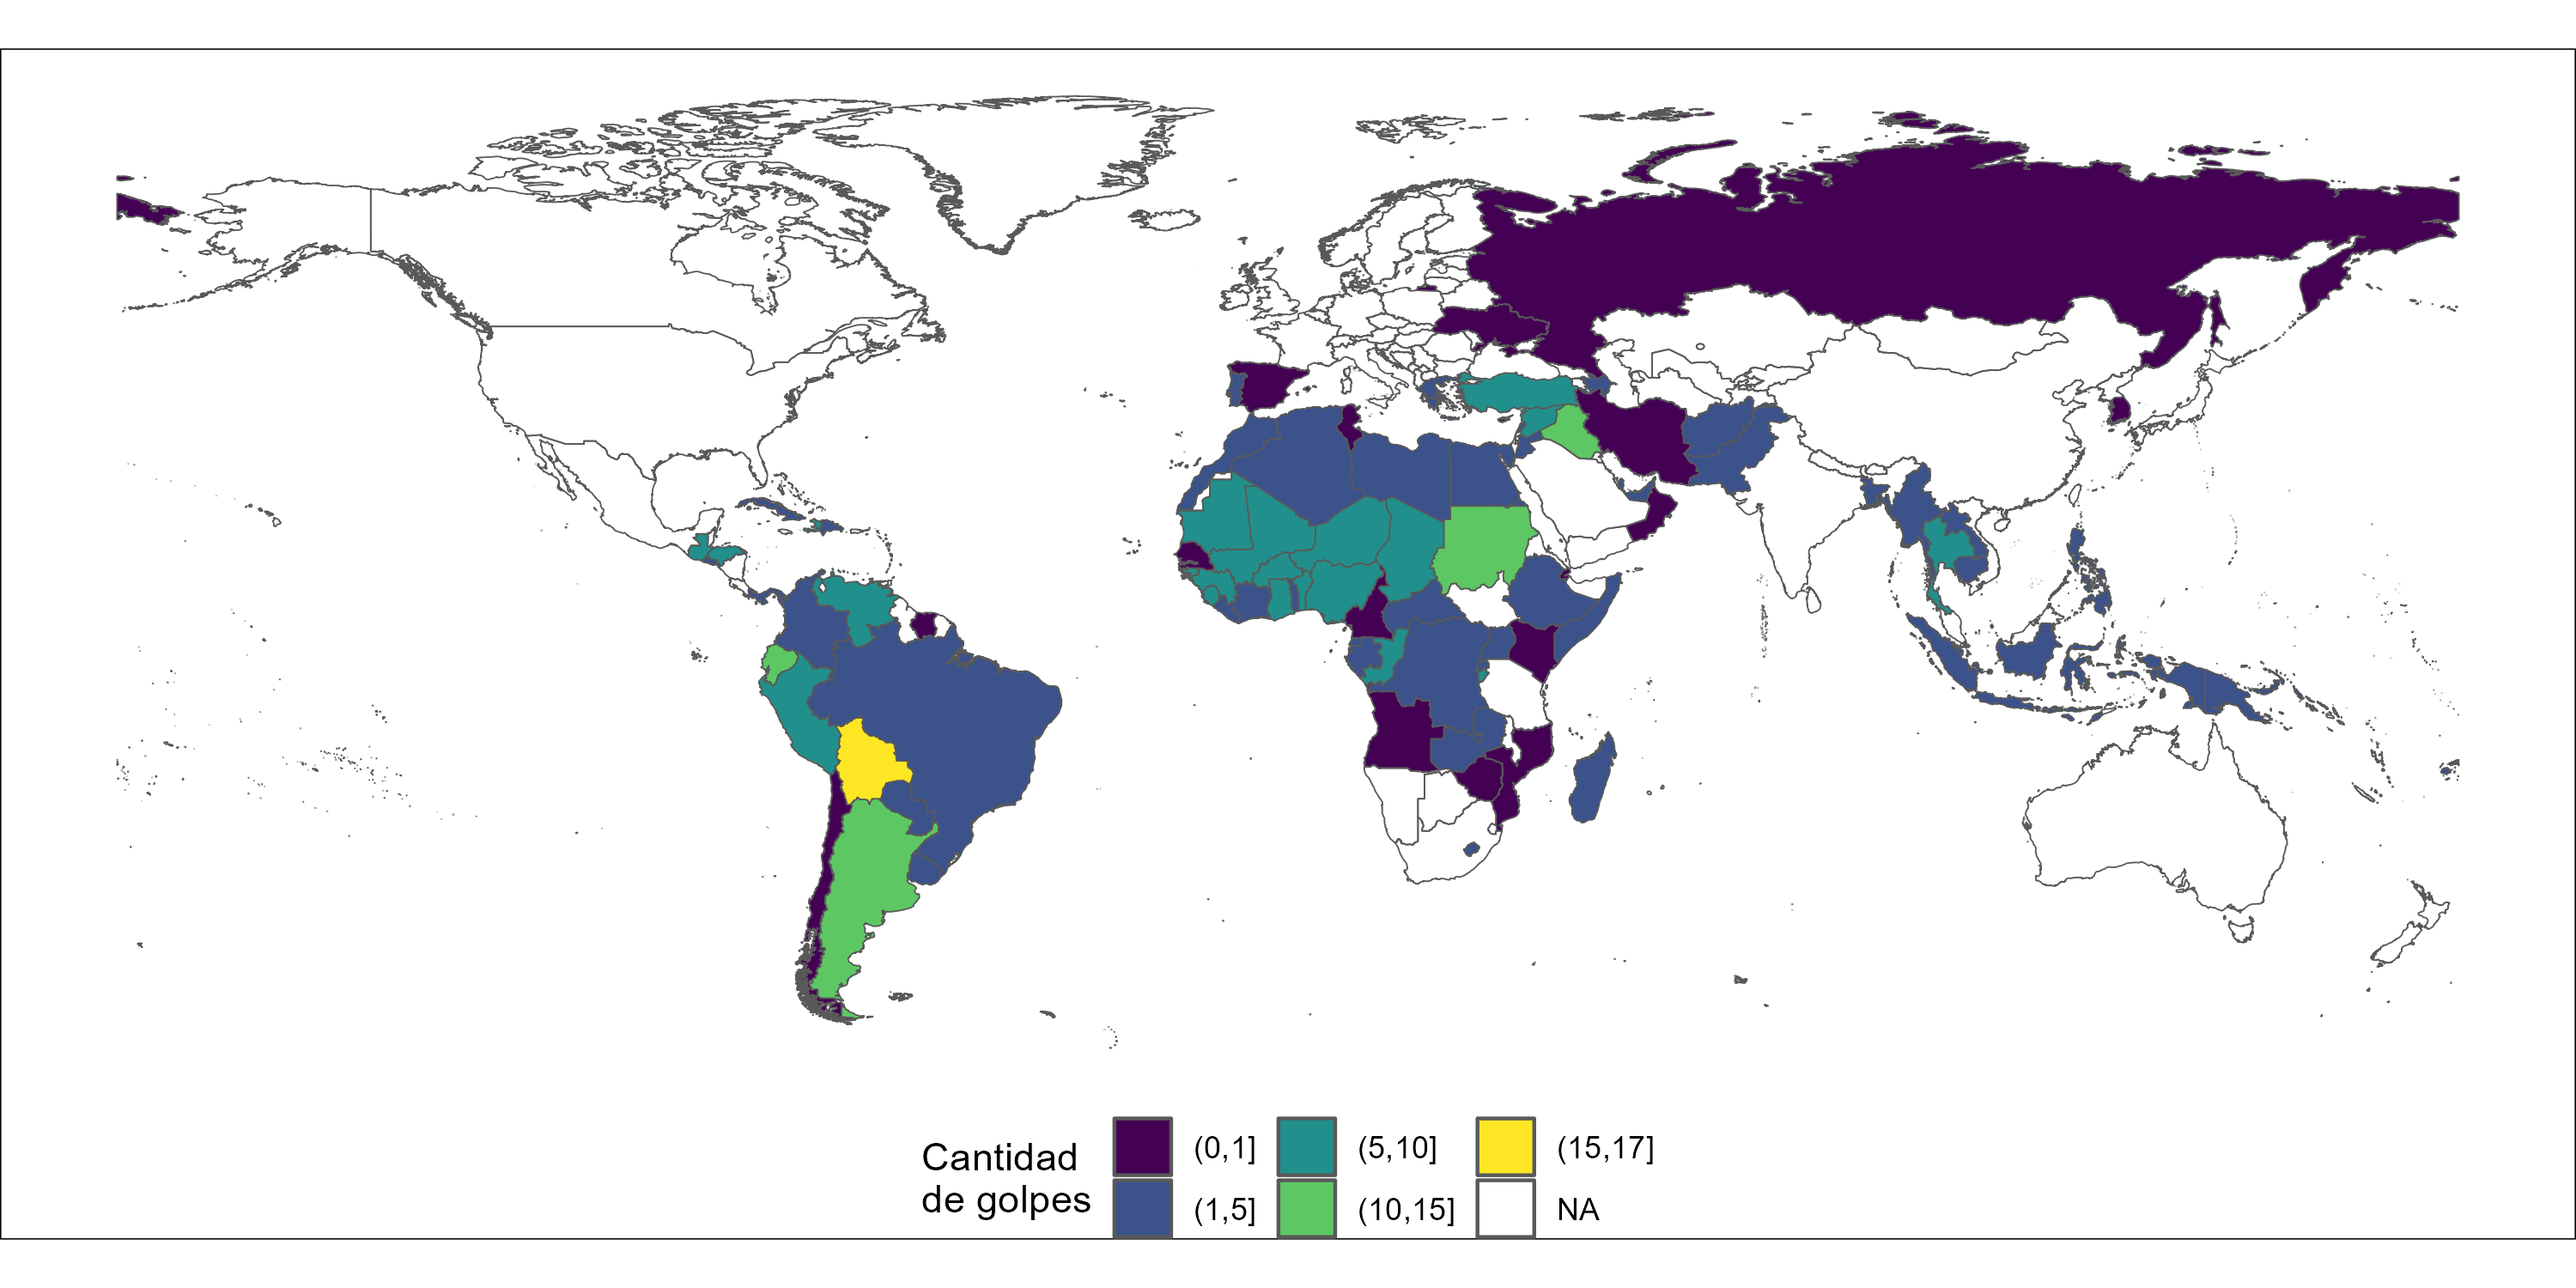
\includegraphics[width=1\textwidth]{2_golpes.png}
  \caption{Conteo de golpes de estado en el mundo}
\end{figure}

\begin{figure}[H]
  \centering  
  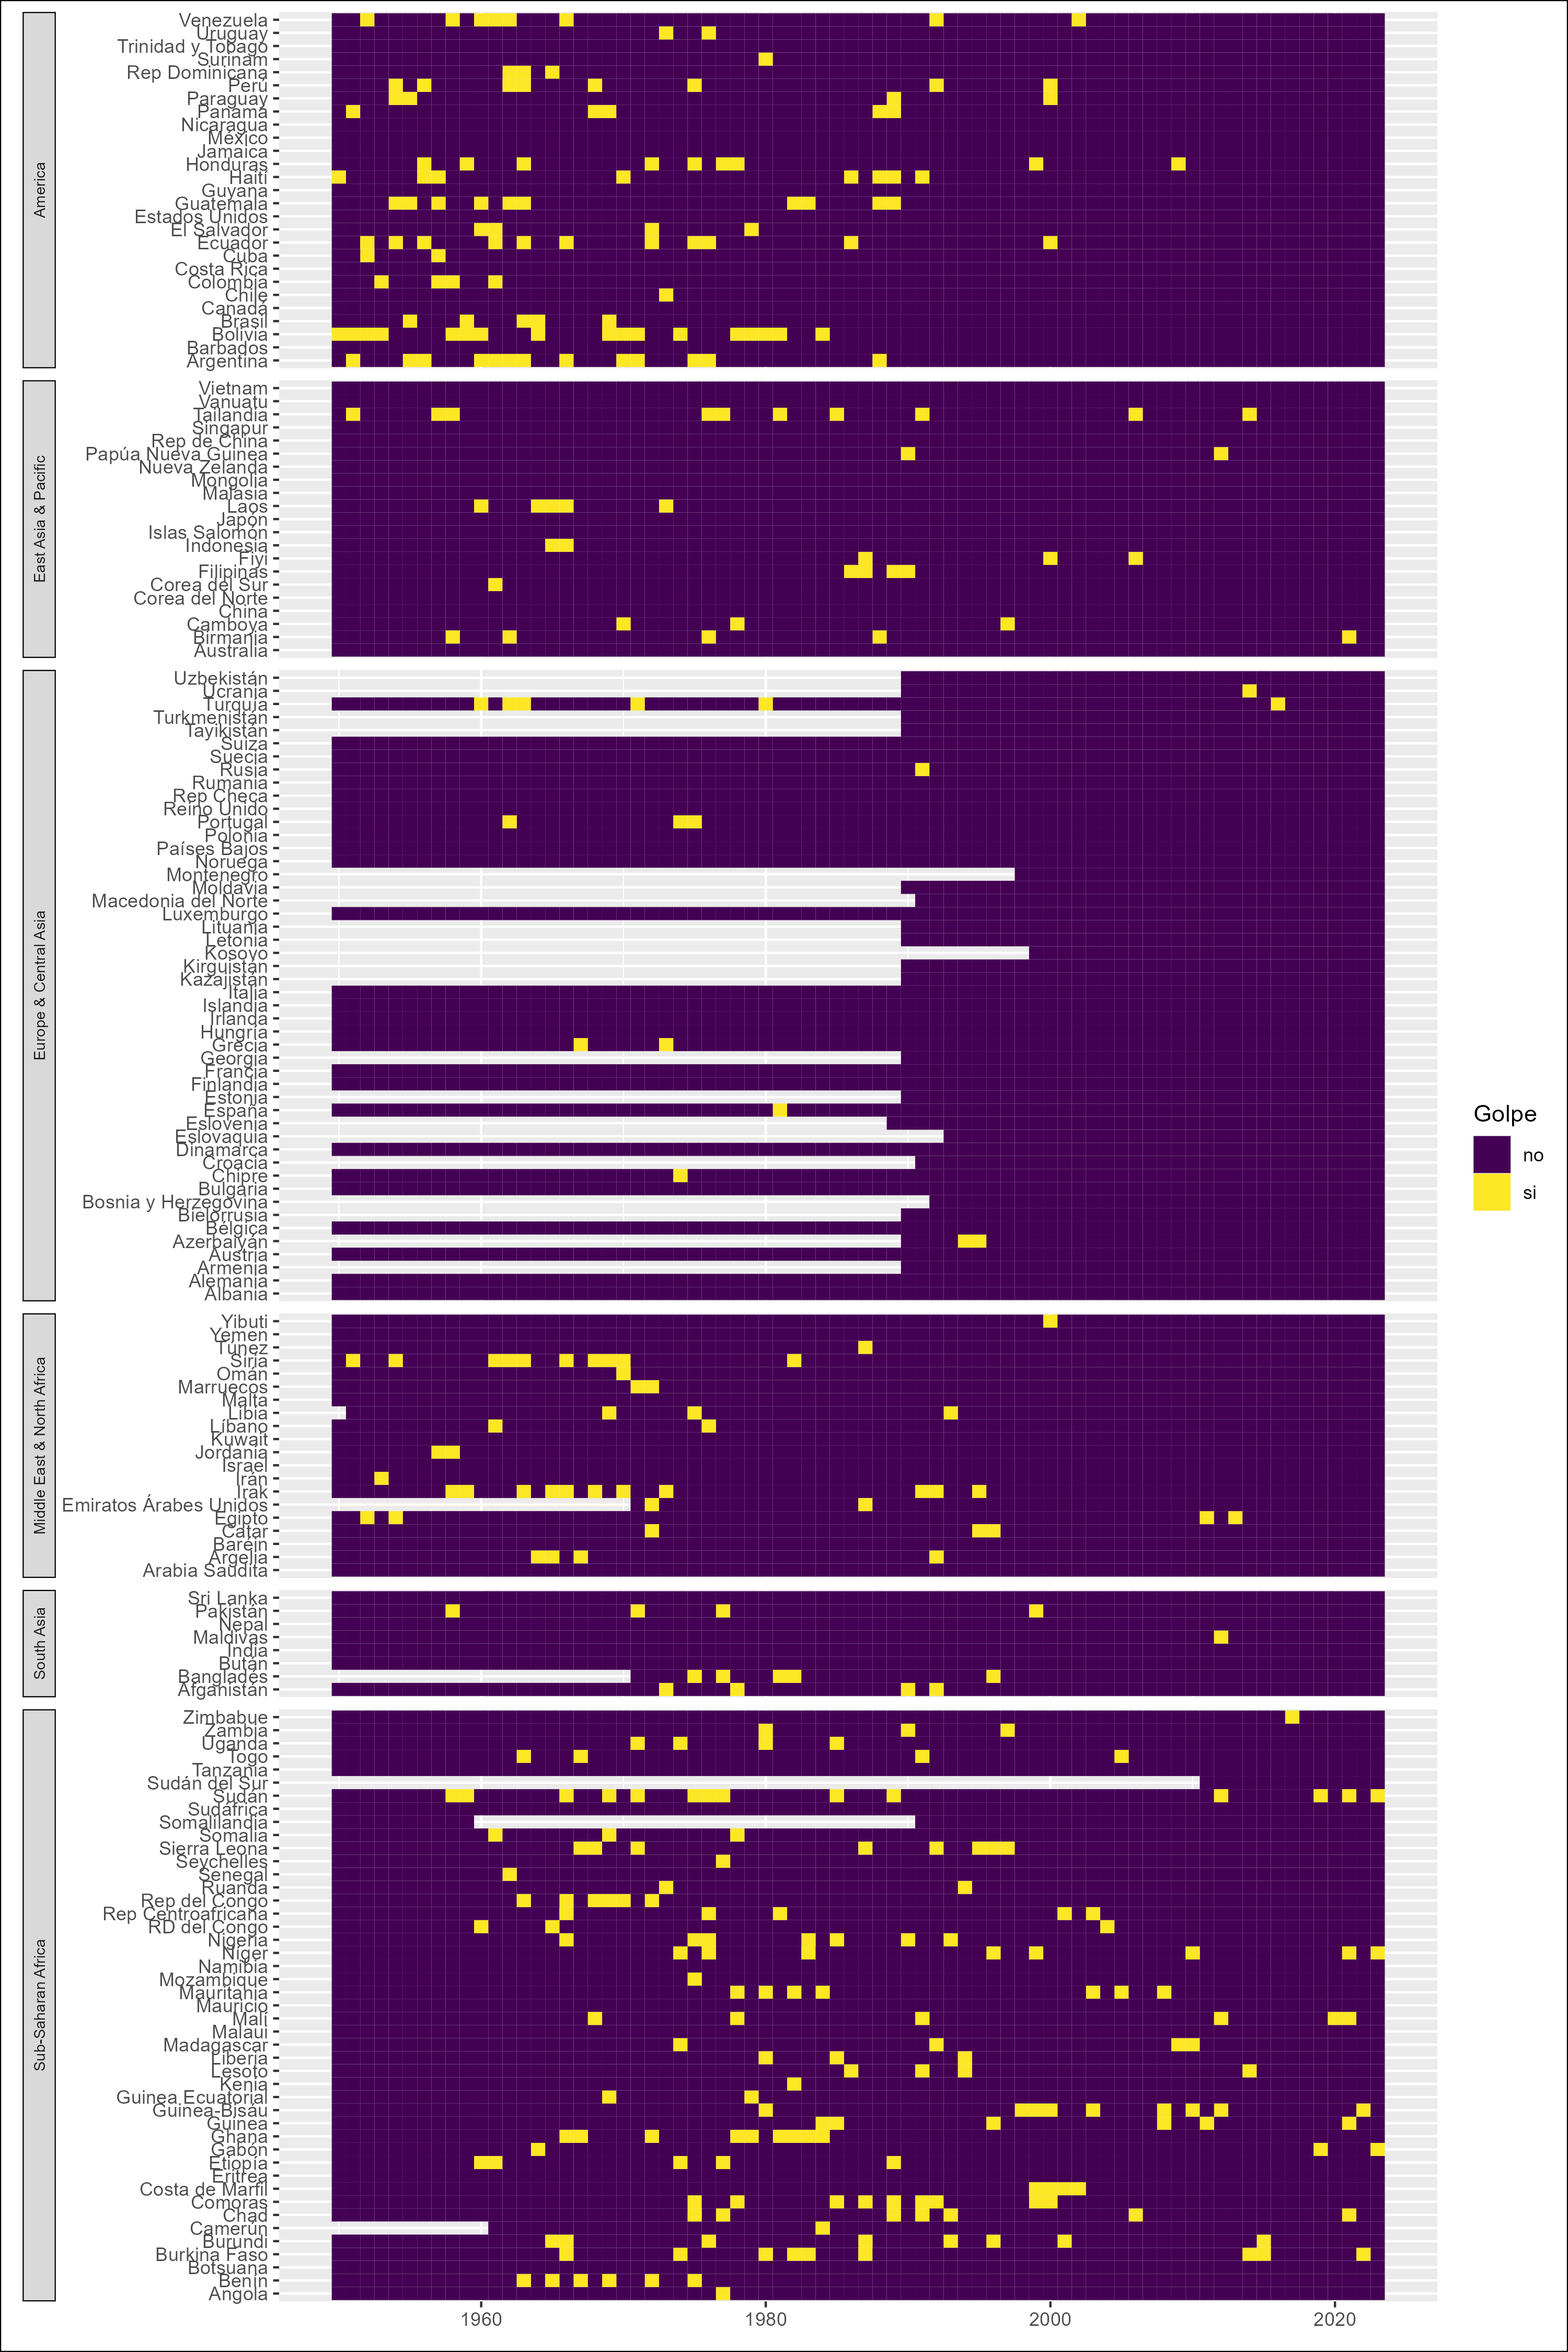
\includegraphics[width=1\textwidth]{3_golpes_anios.png}
  \caption{Conteo de golpes por año y región/país}
\end{figure}


\section{Preprocesamiento de los datos}

\textit{Cargar el dataset con los datos para cada sujeto y los nombres y 
coordenadas de las regiones cerebrales a las que se les registró la actividad. 
Reportar cuántos sujetos y cuántos estados de sueño se observan en el conjunto de
datos.}

\printbibliography

\end{document}